\chapter{Theorie}
%
%
%\section{Theoretische Grundlagen}
%
Im Rahmen dieser Arbeit werden, wenn nicht anders gekennzeichnet, atomare
Einheiten verwendet. Das bedeutet, Energien werden in Einheiten von \\ 1 $E_h$ 
(Hartree) =  2 Rydberg $\approx$ 27.21 eV, Massen in 1 $m_e$, Strecken in 1
$a_0$ und Ladungen in Einheiten von 1 $e$ angegeben.
%
%
%
\section{System}\label{sec:System}
%
Untersucht wird ein ultrakaltes Zweiteilchensystem.
Stellvertretend für andere Systeme kann das bosonische Zweiatomsystem 
Li$^7$Li$^7$ betrachtet werden. Der Hamilton-Operator 
%
\begin{align}\label{eq:kernHam1}
	\Op{H}=\sum_{i=1}^{2}\Op{T}_{K_i}
		+\sum_{i=1}^{2} \Op{V}_{\text{F}}(\textbf{r}_i)
		+\Op{U}(|\textbf{r}_1-\textbf{r}_2|) 
\end{align} 
% 
beschreibt mithilfe der nicht-relativistischen, stationären Schrödingergleichung
%
\begin{align}\label{eq:algSg1}
	\Op{H}\Ket{\psi} = \text{E} \Ket{\psi}
\end{align}
%
das System. 
$\Op{T}_{K_j}=\frac{1}{2\text{M}}\nabla^2_{r_j}$\
ist der 
Kinetische-Energieoperator des jeweiligen Kerns. $\Op{V}_\text{F}$ beschreibt 
ein
Fallenpotential, welches in dieser Arbeit als isotrop und harmonisch angenommen 
wird, das 
heißt 
%
\begin{align}
\Op{V}_\text{F}(\text{r}_i) = \frac{1}{2}\,\text{M}\,\omega^2\, 
\textbf{r}^2_i=\frac{1}{2}\,\text{M}\,\omega^2 \rl{ \, \text{x}^2_i + 
\text{y}^2_i + 
\text{z}^2_i\, } \quad.
\end{align}
%. 
$\Op{U}$  ist eine aus 
Elektronenstrukturrechnung oder Experimenten bekanntes oder motiviertes  
effektives Wechselwirkungspotential. Für Li$^7$Li$^7$ ist in 
\cite{phdthesis:sergey} und den darin enthaltenden Referenzen ein 
solches Potential stückweise zusammengestellt worden, das 
in Grafik 
\ref{pic:NP} dargestellt ist. \\
 
%
%\begin{figure}[t] \centering
%	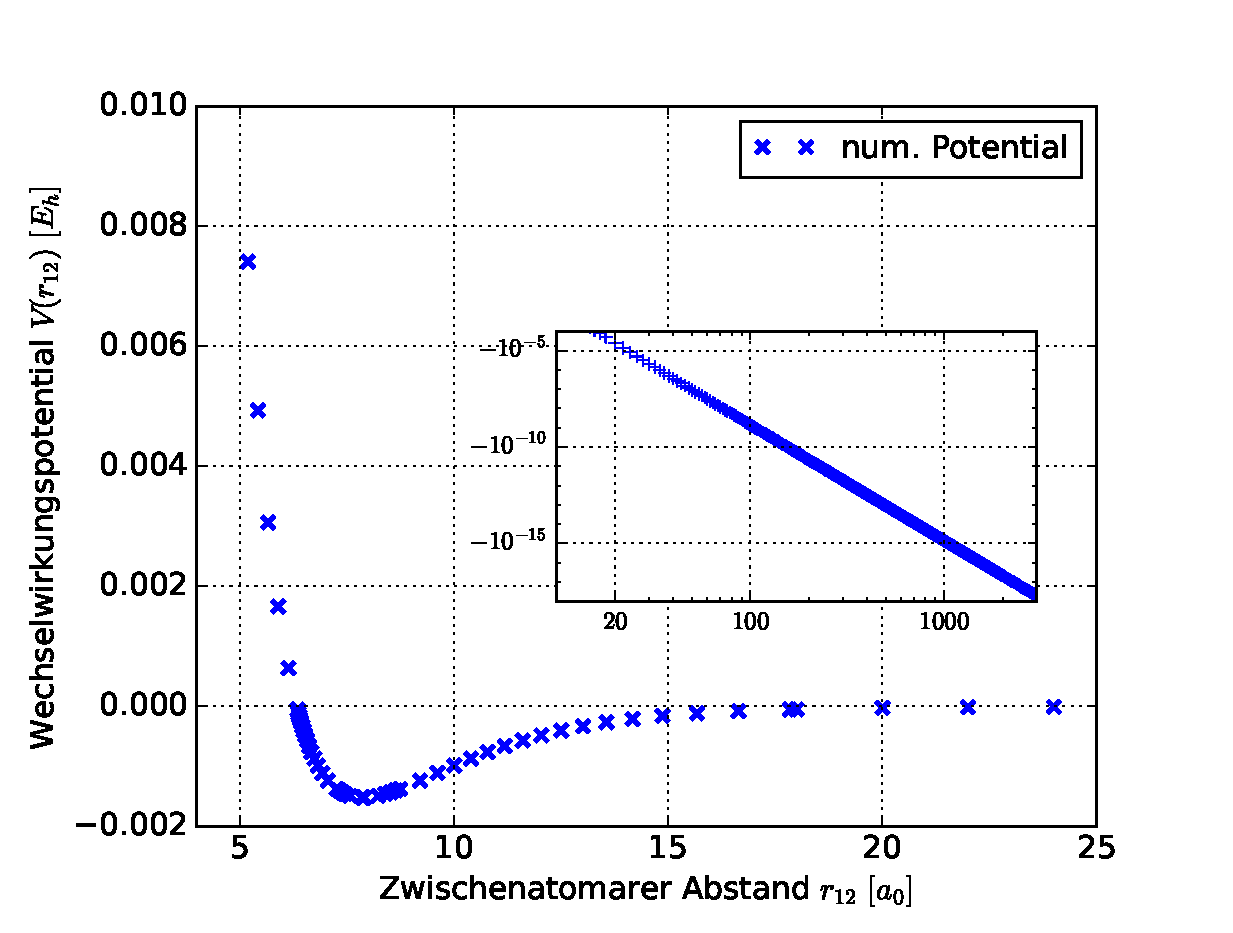
\includegraphics[scale=0.65]{NP.eps}
%	%	\vspace*{-10mm}
%	\caption{Dargestellt ist ein numerisches 
%	Wechselwirkungspotential (gekreuzt) eines 
%		angeregten Tripletzustandes des 
%		$^7$Li$^7$Li Systems.}
%	%\vspace{2mm} %\hrule 
%	\label{pic:NP} 
%\end{figure}
%
Eine mögliche experimentelle Vorlage für ein Zweiatomsystem ist 2011  
realisiert worden \cite{av:7a}.
 Hier handelt es sich um eine
optische Dipolfalle, welche in erster Ordnung auch durch ein quadratisches
Potential beschrieben werden kann  \cite{phdthesis:sala}.  Die ermittelte 
effektive Fallenfrequenz liegt in der Größenordnung von
$10^{4}$ Hz $\approx$ $10^{-13}\ \omega_0$ in atomaren Einheiten. 
% 
\pagebreak
%
%
%
\section{Konfigurationswechselwirkungsrechnung}
%
Da \ref{eq:algSg1} im Allgemeinen nur schwer zu lösen ist, kann nun eine aus der
Quantenchemie (siehe z.B. \cite{b:3a}) bekannte Lösungsmethode herangezogen 
werden:
die Konfigurationswechselwirkungsrechnung (CI). Dazu wird die Wellenfunktion in 
einer endlichen Basis $\Ket{\psi_n}$  
entwickelt    
%
\begin{align}\label{eq:CI-Ansatz}
	\Ket{\psi} \approx \sum_n^N c_n \Ket{\psi_n} \quad.
\end{align}
%
Anschließend wird $\Bra{\psi_i}$ an Gleichung \ref{eq:algSg1} multipliziert. Es 
entsteht das 
Eigenwertproblem
%
\begin{align}\label{eq:EWP}
	\textbf{H}\textbf{c}=E\cdot \textbf{S}\textbf{c}
\end{align}
%
mit 
%
\begin{align}\label{eq:Matrixelemente}
	H_{ij}&=\Bra{\psi_i} \Op{H}\Ket{\psi_j}\\
	S_{ij}&=\braket{\psi_i}{\psi_j} \quad .
\end{align}
%
Wäre die Entwicklung \ref{eq:CI-Ansatz} unendlich und der Basissatz vollständig,
wäre dieser Ansatz exakt. Die Matrix \textbf{S} beinhaltet den sogenannten 
Überlapp der Basisfunktionen. Sind diese orthogonal, so entspricht \textbf{S} 
einer Einheitsmatrix.  Weiterhin wird angenommen, dass sich die 
Basiswellenfunktionen als Produkt der 
Einteilchenwellenfunktionen
beschreiben lassen.

Um die Matrixelemente zu berechnen, müssen 
sechsdimensionale Integrale gelöst werden.%TODO der Satz kommt aus dem nichts, 
%vlt weg lassen
%
%
%
\section{Methodik}
%
%
%
\subsection{Ansatz}
%
Als Ansatz für die oben erwähnten Basisfunktionen werden sogenannte Kartesische-
Gauß-Funktionen bzw. "gaussian-typ orbitals"\ kurz GTOs verwendet. Dieser Ansatz
entstammt der Arbeit von Boys in den 1950er Jahren \cite{av:5a} und ist heute
Standard bei der Elektronenstrukturrechnung (siehe z.B.: \cite{b:3a},
\cite{b:2a}). Die Wellenfunktion in der Ortsdarstellung wird 
also in
Termen von 
%
\begin{align}
\braket{\textbf{r}}{\psi_n}=\psi_n^a(\textbf{r}_1)\cdot\psi_n^c(\textbf{r}_2)
\end{align}
%
mit je
%
\begin{align}\nonumber
\psi_n^a(i,k,m,a,\textbf{A},\textbf{r})&=N_{ikm}(a)\cdot (x-A_x)^i\cdot 
(y-A_y)^k\cdot (z-A_z)^m\  \cdot\\ \label{eq:Produktansatz}
& \qquad \cdot \exp\rl{-a\cdot 
	\rl{(x-A_x)^2+(y-A_y)^2+(z-A_z)^2}}\\\nonumber
%
&= N\cdot x_A^iy_A^kz_A^m\cdot e^{-a r_A^2}\\\nonumber
&= \psi_n^a(\textbf{r})
\end{align}
%
entwickelt. $N$ ist ein Normierungsfaktor und lässt sich mithilfe von 
%
\begin{align}\label{eq:NORM}
	N_{ikm}(a)=\rl{\frac{2a}{\pi}}^\frac{3}{4}\frac{(4a)^\frac{i+k+m}{2}}{\sqrt{(2i-1)!!\cdot(2k-1)!!\cdot(2m-1)!!}}
\end{align}
%
berechnen (vgl. \cite{av:2a}), wobei dieser auch weggelassen werden kann, wobei 
man dann von nicht normierten GTOs spricht.\ \textbf{A} ist 
das 
Zentrum der Gauß-Funktion. Die natürlichen Zahlen ($i,k,m$) geben das 
assoziierte Orbital an. So entspricht zum Beispiel das Tupel (0,0,0) einem 
s-Orbital und (1,0,0) einem p-Orbital in x-Richtung.\\
Um die Matrixelemente \ref{eq:Matrixelemente} ermitteln zu können, müssen 
Einteilchenintegrale
%
\begin{align}\label{eq:1T-Integrale}
\Bra{\psi_i}\Op{O}(\textbf{r}_1)\Ket{\psi_j}  = 
\int  d\textbf{r}_1 
(\psi_i^{a}(\textbf{r}_1) )^*
f(r_1) 
\psi_j^b(\textbf{r}_1)
\end{align}
%
und Zweiteilchenintegrale des Typs
%
\begin{align}\label{eq:2T-Integrale}
I=\Bra{\psi_i}\Op{O}(|\textbf{r}_1-\textbf{r}_2|)\Ket{\psi_j} = \int 
\int\ 
d\textbf{r}_1\ d\textbf{r}_1 
(\psi_i^a(\textbf{r}_1)\psi_i^c(\textbf{r}_2))^* f_{12}(r_{12}) 
\psi_j^b(\textbf{r}_1)\psi_j^d(\textbf{r}_2)
\end{align}
%
zu verschiedenen Operatoren $\Op{O}$ bzw. Funktionen $f$ berechnet werden. Für 
obere Einteilchenintegrale \ref{eq:1T-Integrale} gibt es bereits Algorithmen, 
die effizient implementiert werden können. Die Zweiteilchenintegrale stellen 
dagegen einen größeren Rechenaufwand dar. Anzumerken ist hier, dass die in 
\ref{eq:2T-Integrale} einzusetzenden GTOs prinzipiell unterschiedliche 
Zentren 
haben können. Man spricht hierbei auch von einem 4-Zentrenintegral über GTOs.
%
%
%
\subsection{Berechnung von Zweiteilchenintegralen}\label{sec:Algorithmus}
%
Der in diesem Kapitel vorgestellte Algorithmus entstammt der Veröffentlichung 
\cite{av:1a}. Anders als in dieser Arbeit wird er dort zur Berechnung von 
Zweielektronenintegralen im Rahmen von Elektronenstrukturrechnungen an 
Molekülen verwendet. Weiterhin werden sechs spezielle Fälle für den Integranten 
dargestellt. Für diese Arbeit reicht es aus, den dritten Fall 
(kernal function 3, $k_3(r_{12})$) zu betrachten.\\ 
%
Zur Ableitung des Algorithmus werden vier Schritte der Umformung des Integrals 
vorgenommen. 
%
%
%
\subsubsection{McMurchie-Davidson Schema}
%
Im Abschnitt II.B. von \cite{av:1a} folgt man dem McMurchie-Davidson Schema. 
Dieses entstammt der Arbeit \cite{av:2a} und nutzt aus, dass sich ein Produkt 
aus je zwei Gauß-Funktionen um die Punkte \textbf{A} bzw. \textbf{B} als neue 
Gauß-Funktion 
um einen Punkt \textbf{P} auf der Strecke $\overline{\textbf{AB}}$ schreiben 
lassen. In Abbildung \ref{pic:1d_GTO} ist eine eindimensionale Darstellung 
eines solchen Produkts dargestellt. 
%
%\begin{figure}[H] \centering
%	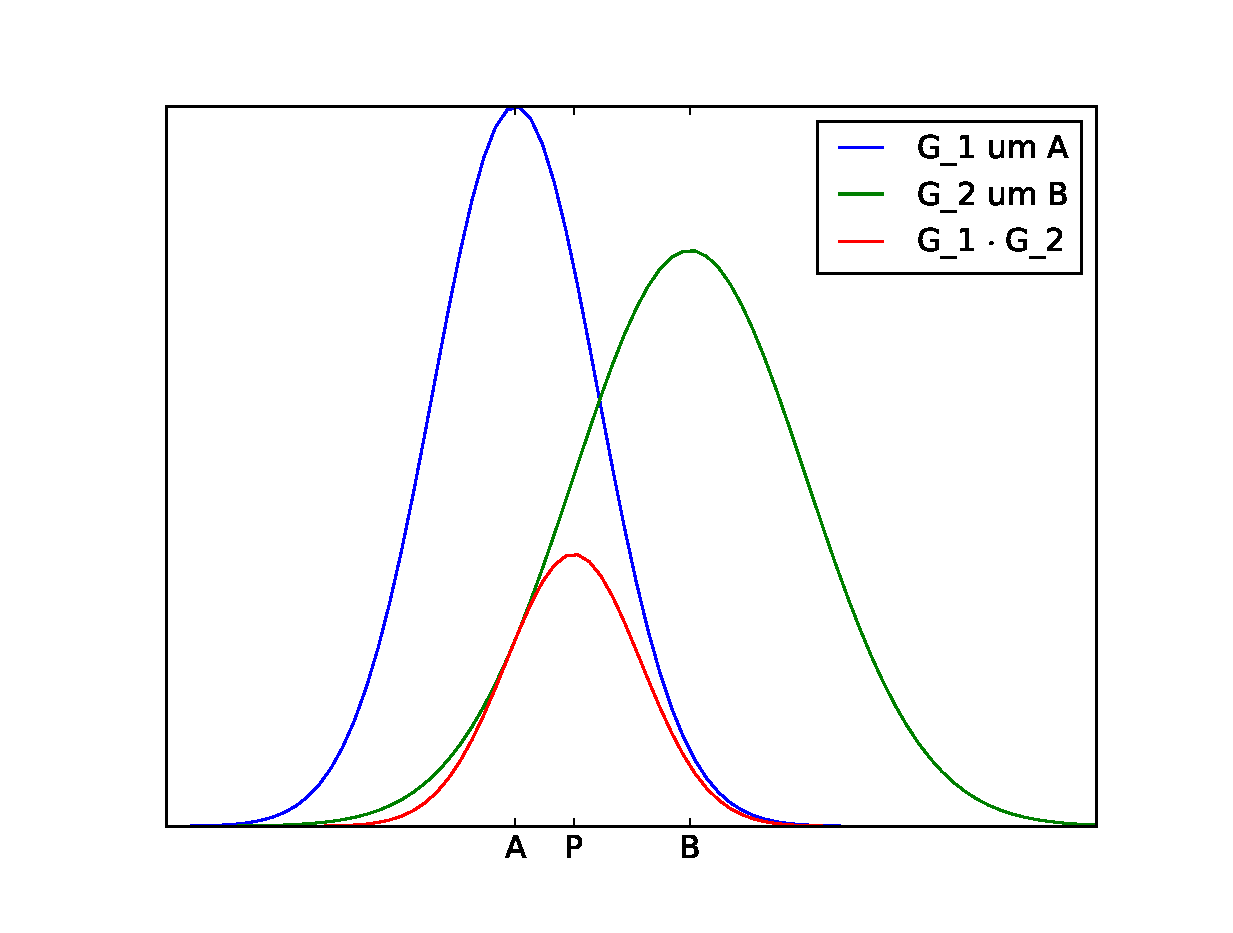
\includegraphics[scale=0.6]{GF.eps}
%	\vspace*{-7mm}
%	\caption{Eindimensionales Beispiel für das Produkt zweier beliebiger 
%	Gauß-Funktionen (vgl. \ref{eq:Produktansatz}). Die Lage des neuen Maximas 
%	ergibt sich durch 
%	\ref{eq:neuesZentrum_P}.}
%	\label{pic:1d_GTO} 
%\end{figure}
%
Dieses Vorgehen lässt sich beliebig oft wiederholen, was ein 
besonderer Vorteil für die oben erwähnten 4-Zentrenintegrale darstellt. Das 
Produkt von zwei nicht normierten GTOs lässt sich in eine 
Summe
%
\begin{align}
\psi_a(\textbf{r}_1)\cdot \psi_b(\textbf{r}_1) &=  x_A^i\,y_A^k\,z_A^m\cdot  
x_B^j\,y_B^l\,z_B^n\cdot e^{-b r_B^2-a 
		r_A^2}\\
%
&= \sum_{t=0}^{i+j}E^{i,j}_t\ 
\sum_{u=0}^{k+l}E^{k,l}_u\ \sum_{v=0}^{m+n}E^{m,n}_v\ 
\Lambda_{tuv}(\textbf{r}_1,p,\textbf{P})
\end{align}
%
über
%
\begin{align}
\Lambda_{tuv}(\textbf{r}_1,p,\textbf{P})&=\frac{\text{d}^t}{\text{d}P_x^t}\frac{\text{d}^u}{\text{d}P_y^u}\frac{\text{d}^v}{\text{d}P_z^v}\
 \exp(-p r_{1,P}^2)
\end{align}
%
schreiben.
Die nötigen Koeffizienten werden 
rekursiv mithilfe von
%
\begin{align}\label{eq:E:coef1}
E_0^{0,0}&=\exp(-\frac{ab}{p}(A_x-B_x)^2)\\\label{eq:E:coef2}
E_0^{i+1,j}&=-\frac{b}{p}(A_x-B_x)E^{i,j}_0 + E_1^{i,j}\\\label{eq:E:coef3}
E_0^{i,j+1}&=\frac{a}{p}(A_x-B_x)E^{i,j}_0 + E_1^{i,j}\\\label{eq:E:coef4}
E_t^{i,j} &= \frac{1}{2pt}\rl{iE^{i-1,j}_{t-1}+jE^{i,j-1}_{t-1} }
\end{align}
%
berechnet (siehe z.B. auch \cite{av:3a}), wobei das neue Zentrum durch
%
\begin{align}\label{eq:neuesZentrum_P}
p:=a+b \qquad, \qquad
\textbf{P}:=\frac{a\textbf{A}+b\textbf{B}}{p}
\end{align}
%
bestimmt ist. Eine analoge Umformung kann für das 
zweite Teilchen (\textbf{r}$_2$) mit
%
\begin{align}\label{eq:Q}
q:=c+d \qquad, \qquad
\textbf{Q}:=\frac{c\textbf{C}+d\textbf{D}}{q}
\end{align}
%
durchgeführt werden. Weiterhin zeigt Boys, dass alle Integrale dieses Typs eine 
%TODO ACHTUNG ZEILENTRENNUNG in finaler Version pruefen
|\textbf{P}-\textbf{Q}| Abhängigkeit haben, das heißt, dass sie nicht von den 
einzelnen Komponenten der Vektoren \textbf{P} und \textbf{Q} abhängen. Daher  
gilt 
%
$\rl{\frac{\DEL}{\DEL P_x}}^i = \rl{-\frac{\DEL}{\DEL 
Q_x}}^i=(-1)^i \rl{\frac{\DEL}{\DEL Q_x}}^i$
%
, was für das gesamt Integral bedeutet:
%
\begin{align}\label{eq:E:Koef}
I &= % N_{ikm}(a)N_{jln}(b)N_{i'k'm'}(c)N_{j'l'n'}(d) \cdot \\ 
%& \cdot 
\sum_{t=0}^{i+j}E^{i,j}_t\ \sum_{u=0}^{k+l}E^{k,l}_u\ 
\sum_{v=0}^{m+n}E^{m,n}_v\ (-1)^{t+u+v} \sum_{t'=0}^{i'+j'}E^{i',j'}_{t'}\ 
\sum_{u'=0}^{k'+l'}E^{k',l'}_{u'} \sum_{v'=0}^{m'+n'}E^{m',n'}_{v'}\ 
R^{t+t',u+u',v+v'}\ ,
\end{align}
%
wobei die gestrichenen Indizes für die Potenzen der GTO des 
zweiten Teilchens 
(\textbf{r}$_2$) stehen. Weiterhin wird die Schreibweise
% 
\begin{align}\label{eq:McM-D:kartesieAbleitungen}
R^{\tau,\rho,\sigma}&=\frac{d^\tau}{dQ^\tau_x}\ 
\frac{d^\rho}{dQ^\rho_y}\ \frac{d^\sigma}{dQ^\sigma_z}\ 
B\\\label{eq:basisint1}
B&= \int \int d\textbf{r}_1 d\textbf{r}_2 \ e^{-pr_{1,P}^2} \cdot 
f_{12}(r_{12}) \cdot e^{-qr_{2,Q}^2} \quad.
\end{align}
%
genutzt, wobei $B$ das sogenannte \textit{Basisintegral}  ist. Weiter wird dem 
McMurchie-Davidson Schema nicht gefolgt. 
%
%
%
\subsubsection{Analytische Modifikationen des Basisintegrals}\label{sec:modifik}
%
Als zweiten Schritt vereinfacht \cite{av:1a} das Basisintegral :
\begin{enumerate}
	\item[1.]  Es wird beobachtet, dass ,wie erwähnt, $B$ nur 
	von 
	|\textbf{P}-\textbf{Q}| abhängt. Daher kann nun eine 
	Koordinatenverschiebung 
	vorgenommen werden, sodass sich ein Punkt (z.B. \textbf{P}) im Ursprung 
	befindet\footnote{Im folgenden wird \textbf{Q}$_\text{neu}$ weiterhin mit 
	\textbf{Q} bezeichnet.}.\\
	$\Rightarrow \ \textbf{P}_\text{neu2}=0\ , \qquad 
	\textbf{Q}_{\text{neu}}=\textbf{Q}-\textbf{P}$
	%
	%
	\item[2.] Anschließend wird die noch verschobene Gauß-Funktion in 
	Kugelflächenfunktionen und modifizierte sphärische Besselfunktionen der 
	ersten Art entwickelt. Es gilt:
	\begin{align}
	e^{-qr_{2,Q}^2}=4\pi 
	e^{-qQ^2}\sum_{l=0}^{\infty}i_l(2qQr_2)\sum_{m=-l}^{+l} 
	Y_{lm}^*(\hat{Q})Y_{lm}(\hat{r}_2) \quad,
	\end{align}
	wobei $Q=|\textbf{Q}|$ ist. Diese Gleichung kann durch 
	die Verwendung von zum Beispiel \cite{b:5a} gezeigt 
	werden.
	Da über den gesamten Raum integriert wird, entfallen aus  
	Symmetriegründen 
	alle Terme außer l=0 ($\rightarrow$ m=0). Daher verbleibt B bei
	\begin{align}\label{eq:Basisintegral:zwerg}
	B=e^{-qQ^2} \int \int d\textbf{r}_1 d\textbf{r}_2\ e^{-pr_1^2-qr_2^2} 
	\frac{\sinh(2qQr_2)}{2qQr_2}\cdot f_{12}(r_{12}) \quad .
	\end{align}
	%
	%
	\item[3.] Als letzte Umformung wird eine Koordinatentransformation 
	durchgeführt. Hierbei geht man in ein System, indem ein Teilchen  im 
	Ursprung und das zweite auf der z-Achse liegt. Anschließend geht man in 
	Kugelkoordinaten. Die daraus resultierende Integralbildung wird z.B. in 
	\cite{av:6a} beschrieben. 
	%
	\begin{align*}
	\{x_1,y_1,z_1,x_2,y_2,z_2\}\rightarrow\{r_1,r_2,r_{12},\alpha,\beta,\gamma\}
	\end{align*}
	%
	
	$\alpha,\beta$ und $\gamma$ sind resultierende Eulerwinkel, die entstehen, 
	wenn das Koordinatensystem 1 (\textbf{r}$_1$) derart 
	gedreht wird, dass 
	der Vektor \textbf{r}$_2$ auf der z-Achse liegt. 
	Weiterhin muss erwähnt werden, dass offensichtlich d\textbf{r}$_1$ = 
	d\textbf{r}$_{12}$ gilt, wodurch sich im Gegensatz zu \cite{av:6a} die 
	Bedeutung von $r_1$ und	$r_{12}$ vertauscht. 
	Da außerdem $r_1=|\textbf{r}_{12}+\textbf{r}_2|$ gilt, 
	folgt nach elementarer Winkelintegration für allgemeine Funktionen f,g und 
	h:
	\footnote{$\textbf{r}_1=\textbf{r}_{12}+\textbf{r}_{2},\ 
		r_1=\sqrt{r_{12}^2+r_2^2-2r_{12}r_2\cos(\beta)},\ 
		d\textbf{r}_{12}= r^2_{12} \sin(\beta) \ dr_{12}\ d\alpha\ d\beta$} 
%
	\begin{align}\nonumber
		\int \int & f(r_{1}) g(r_2)h(r_{12}) d\textbf{r}_1d\textbf{r}_2 =\\
		% 
		& 8\pi^2\int_{0}^{\infty}h(r_{12})\ r_{12}\ dr_{12}\int_{0}^{\infty} 
		g(r_2)\ r_2\ dr_2 \int_{|r_{12}-r_2|}^{r_{12}+r_2}f(r_{1})\ r_{1}\ 
		dr_{1}\quad.
	\end{align}
	Nach Integration (vergleiche \ref{eq:Basisintegral:zwerg} ) über $r_1$ und 
	$r_2$ verbleibt
	\begin{align}\label{eq:B:zwischenErg}
		B= \sqrt{\frac{\pi^5}{p+q}}\frac{1}{pq}\cdot \int_{0}^{\infty}dr_{12}\ 
		f_{12}(r_{12})\cdot r_{12}\cdot \rl{\frac{e^{-  
		\frac{pq}{p+q}(r_{12}-Q)^2}-e^{-\frac{pq}{p+q}(r_{12}+Q)^2}}{Q}}\quad .
	\end{align}
\end{enumerate} 
%
Im Folgenden wird die zusammenfassende Größe
%
\begin{align}
\xi := \frac{p\cdot q}{p+q}
\end{align}
%
verwendet, um \ref{eq:B:zwischenErg} zu vereinfachen.
%
%
%
\subsubsection{Hobson Theorem und 
Schlegel-Koeffizienten}\label{sec:Hobson_schlegel}
%
Wie in \ref{eq:McM-D:kartesieAbleitungen} zu erkennen ist, müssen  
Ableitungen des Basisintegrals berechnet werden\footnote{In der Arbeit 
\cite{av:9a} ist eine genauere und z.T. berichtigte Version dieses Teils des 
Algorithmus aus \cite{av:1a} beschrieben.}. Da B nur von $Q=|Q|$ abhängt, 
ist es sinnvoll, die kartesischen Ableitungen in sphärische Ableitungen nach 
$Q$ umzuformen.\\
Dazu wird als Erstes auf die Arbeit \cite{av:4a} verwiesen, in der ein 
vollständiger, analytischer Ausdruck für die Umformung von sphärische in  
kartesische GTOs (Koordinatenwechsel des polynomartigen Anteils) präsentiert 
wird. Die Rückumformung, das heißt die Umformung von kartesischen in 
sphärische Koordinaten, kann nach Absprache mit den Autoren von \cite{av:1a} 
wie folgt dargestellt werden. Sind $c_{l_xl_yl_z}^{l,m}$ die reellen 
Schlegel-Koeffizienten aus \cite{av:4a}, so können die Koeffizienten der 
Rückumformung mit
%
\begin{align}\nonumber
c^{-1}(l,m,l_x,l_y,l_z)&=\frac{2}{\Gamma\rl{\frac{l_x+l_y+l_z+l+3}{2}}} 
 \ \cdot \\ \label{eq:def:c_koef}
 &\cdot  \sum_{a+b+c\leq l} c_{l_xl_yl_z}^{lm}\cdot 
\Gamma\rl{\frac{1+l_x+a}{2}}\cdot 
\Gamma\rl{\frac{1+l_y+b}{2}}\cdot \Gamma\rl{\frac{1+l_z+c}{2}}
\end{align}
%
berechnet werden. Damit ist also die Umformung
%
\begin{align}\label{eq:trafo_c-1}
x^{l_x}y^{l_y}z^{l_z} = \sum_{l=0}^{l_{max}}\sum_{m=0}^l 
c^{-1}(l,m,l_x,l_y,l_z)\cdot r^{l_{max}-l} Z_{lm}(\textbf{r})
\end{align}
%
möglich. $Z_{lm}(\textbf{r})=r^l\cdot Y_{lm}(\hat{\textbf{r}})$ sind die 
reellen, soliden 
Kugelflächenfunktionen ohne Racah's Normalisierung und 
$l_{max}=l_x+l_y+l_z$. Eine detailliertere Beschreibung inkl. aller 
Definitionen bzgl. dieser Transformation ist im Anhang 
\ref{sec:AnhangA:Schlegel} zu finden. Weiterhin sei erwähnt, 
dass auch 
\cite{av:4a} einige kleinere Tippfehler hat, welche in Anhang berichtigt sind.\\

Analog dazu können mithilfe der selben Koeffizienten auch die 
Differenzialoperatoren \ref{eq:McM-D:kartesieAbleitungen} umgeformt werden. 
Mit der Verwendung des Hobson Theorems in der Form
%
\begin{align}\label{eq:Hobson}
\Op{Z}_{lm}(\nabla_Q)g(Q)=\left[\mathcal{D}^l_Qg(Q)\right]Z_{lm}(\textbf{Q}) 
\end{align}
%
können die kartesischen Ableitungen durch 
%
\begin{align}
R^{\tau,\rho,\sigma}=\frac{d^\tau}{dQ^\tau_x}\ 
\frac{d^\rho}{dQ^\rho_y}\ \frac{d^\sigma}{dQ^\sigma_z}\ 
B=\sum_{l=0}^{l_{max}}\sum_{m=-l}^{l}c^{-1}(l,m,\tau,\rho,\sigma)\cdot
 \nabla_Q^{l_{max}-l}\left[(\mathcal{D}_Q^lB)Z_{lm}(\textbf{Q})\right]
\end{align}
%
ausgedrückt werden, wobei $\mathcal{D}^l_Q=Q^{-1}\DEL_Q$ darstellt. Ist  
$l_{max}-l$ 
ungerade, so ist $c^{-1}=0$. Mithilfe der Relation 
$\nabla_Q^2=Q^2\mathcal{D}^l_Q+3\mathcal{D}_Q$ 
kann nun \ref{eq:McM-D:kartesieAbleitungen} in die finale Form
%
\begin{align}\label{eq:final:Hobson}
R^{\tau,\rho,\sigma}=\sum_{l=0}^{l_{max}}\sum_{m=-l}^{l}c^{-1}(l,m,\tau,\rho,\sigma)Z_{lm}(\textbf{Q})
 \sum_{k=0}^{k_{max}}d_k^{l,k_{max}} \cdot 
\left[(\mathcal{D}_Q^{l_{max}-k}B)\right]Q^{l_{max}-l-2k}
\end{align}
%
geschrieben werden. Hierbei ist $k_{max}=\frac{1}{2}(l_{max}-l)$ und die 
Koeffizienten $d_k^{l,k_{max}}$ können rekursiv berechnet werden:
%
\begin{align}\nonumber
d_n^{l,m}=d_n^{l,m-1} &+\left[2l+3+4(m-n)\right]d_{n-1}^{l,m-1}+\\ 
\label{eq:rek_d}
&2(m-n+1)(2l+3+2(m-n))d_{n-2}^{l,m-1} \qquad.
\end{align} 
%
Die Rekursion startet bei $d_{-1}^{l,m}=0$ und $d_0^{l,m}=1$.
%
%
%
\subsubsection{Radiale Ableitungen der Basisintegrale}
%
Der letzte in der Arbeit \cite{av:1a} präsentierte Schritt 
sieht die 
Evaluation der radialen Ableitungen des Basisintegrals vor. Dazu werden zwei 
Vorgehensweisen dargestellt. Die erste in der vorliegenden 
Arbeit nicht 
behandelte Vorgehensweise nutzt eine Taylorentwicklung\footnote{In den Formeln 
(44)-(46) von \cite{av:1a} ist bei der Umformung der Exponentialfunktionen in 
den sinh ein Faktor 2 verlorengegangen. Weiterhin fehlt im 
ersten Term von 
(47) ein weiterer Faktor 2.} von $Q$ um 0 aus. Da im Regime der ultrakalten 
Gase der Bereich von sehr kleinen Teilchenabständen ($Q$) eher uninteressant 
ist\footnote{Da in diesem Bereich die harmonische Falle vernachlässigt werden 
kann und die Schrödingergleichung in Relativ- und Schwerpunktkoordinaten 
separiert und somit in 1D lösbar ist.}, wird nun das zweite Vorgehen für 
mittlere und große $Q$ erläutert.\\

Das Basisintegral \ref{eq:Basisintegral:zwerg} kann in zwei Terme 
geschrieben werden. Mithilfe der Definition 
%
\begin{align}
\mathcal{H}^\pm_{jkl}&:=\sqrt{\frac{\pi^5}{p+q}}\frac{1}{pq} \int_{0}^{\infty} 
dr_{12}\ r_{12}^j\ \cdot 
\rl{\frac{1}{Q}\frac{\text{d}}{\text{d}Q}}^l\rl{\frac{e^{-\xi(r_{12}\pm 
			Q)^2}}{Q^k}}
\end{align}
%
gilt
%
\begin{align}\label{eq:diff_op}
\mathcal{D}_Q^lB=\left[\rl{\frac{1}{Q}\frac{d}{dQ}}^lB\right] 
=\rl{\mathcal{H}^-_{11l}-\mathcal{H}^+_{11l}} \quad .
\end{align}
%
Durch abermalige Anwendung des Differentialoperators $\mathcal{D}_Q$ kann die 
Rekursion
%
\begin{align}\label{eq:rek:H}
\mathcal{H}_{jkl}^{\pm} = \mp 2\xi\cdot \mathcal{H}_{j+1,k+1,l-1}^\pm-2\xi\cdot 
\mathcal{H}_{j,k,l-1}^\pm-k\cdot\mathcal{H}_{j,k+2,l-1}^\pm
\end{align}
%
gefunden werden. Man beobachtet, dass auf Kosten von j und k der Index l für 
die Ableitungen reduziert werden kann. Durch die trivialen Relationen
\begin{align} \label{eq:prop:H}
\mathcal{H}_{jk0}^{\pm} &= \frac{1}{Q^k} \cdot \mathcal{H}_{j00}^\pm\\ 
\mathcal{H}_{j00}^{\pm} &=\sqrt{\frac{\pi^5}{p+q}}\frac{1}{pq} \cdot \Pi_j^\pm
\end{align}
vereinfacht sich das nun noch zu berechnende Integral auf
\begin{align}\label{eq:PI-Integrale}
\Pi_j^\pm= \int_{0}^{\infty}dr_{12}\ r_{12}^j \cdot f_{12}(r_{12}) \cdot 
e^{-\xi (r_{12} \pm Q)^2}\quad .
\end{align}
%
%
%
\subsubsection{Zusammenfassung}\label{sec:Zusammenfassung:Algorithmus}
%
Ziel des Algorithmus ist es gewesen, 
%
\begin{align}\nonumber
I= \int \int\ 
d\textbf{r}_1\ d\textbf{r}_1 
(\psi_i^a(\textbf{r}_1)\psi_i^c(\textbf{r}_2))^* f_{12}(r_{12}) 
\psi_j^b(\textbf{r}_1)\psi_j^d(\textbf{r}_2)
\end{align}
%
zu berechnen. Mithilfe des Ansatzes der GTOs kann die Integralberechnung   
auf die Schar der $\Pi_j^\pm$ Integrale \ref{eq:PI-Integrale}
%
\begin{align}\nonumber
\Pi_j^\pm= \int_{0}^{\infty}dr_{12}\ r_{12}^j \cdot f_{12}(r_{12}) \cdot 
e^{-\xi (r_{12} \pm Q)^2}
\end{align}
% 
zurückgeführt werden. Wichtig hierbei ist die korrekte Definition von $Q$ 
(\ref{eq:Q}) mit Berücksichtigung der Koordinatenverschiebung in 
\ref{sec:modifik}, bei der P auf den Ursprung verschoben 
wird. Anschließend 
ermittelt man mithilfe der Rekursion \ref{eq:rek:H}
%
\begin{align}\nonumber
\mathcal{H}_{jkl}^{\pm} = \mp 2\xi\cdot \mathcal{H}_{j+1,k+1,l-1}^\pm-2\xi\cdot 
\mathcal{H}_{j,k,l-1}^\pm-k\cdot\mathcal{H}_{j,k+2,l-1}^\pm
\end{align}
%
und den benötigten Proportionalitäten \ref{eq:prop:H} die Integrale 
$\mathcal{H}_{11l}^\pm$. \\
Via \ref{eq:final:Hobson} mit \ref{eq:diff_op}
%
\begin{align}\label{R_sum}
R^{\tau,\rho,\sigma}=\sum_{l=0}^{l_{max}}\sum_{m=-l}^{l}c^{-1}(l,m,\tau,\rho,\sigma)Z_{lm}(\textbf{Q})
\sum_{k=0}^{k_{max}}d_k^{l,k_{max}} \cdot 
\left[(\mathcal{H}^-_{11l}-\mathcal{H}^+_{11l})\right]Q^{l_{max}-l-2k}
\end{align}
%
und \ref{eq:E:Koef} 
%
\begin{align}\nonumber 
I &= %N_{ikm}(a)N_{jln}(b)N_{i'k'm'}(c)N_{j'l'n'}(d) \cdot \\ \nonumber
%& \cdot 
\sum_{t=0}^{i+j}E^{i,j}_t\ \sum_{u=0}^{k+l}E^{k,l}_u\ 
\sum_{v=0}^{m+n}E^{m,n}_v\ (-1)^{t+u+v} \sum_{t'=0}^{i'+j'}E^{i',j'}_{t'}\ 
\sum_{u'=0}^{k'+l'}E^{k',l'}_{u'} \sum_{v'=0}^{m'+n'}E^{m',n'}_{v'}\ 
R^{t+t',u+u',v+v'}
\end{align}
%
ist das Integral berechnet. \\

Dieses Vorgehen ist unabhängig von der Form der eingesetzten Funktion 
$f_{12}(r_{12})$, solange die Abhängigkeit $r_{12}=|\textbf{r}_1-\textbf{r}_2|$ 
stimmt. $\Pi^\pm_j$ kann sowohl analytisch als auch im Allgemeinen numerisch 
gelöst werden. Auf mögliche Probleme dabei wird im folgenden Abschnitt 
eingegangen. Die Normierungskonstanten $N$ können ohne Beschränkung der 
Allgemeinheit auch weggelassen werden. Dies entspricht der Verwendung von 
nicht normierten GTOs als Basisfunktionen.
%
%
%
\subsection{Berechnung der Basisintegrale}
%
Dieser Abschnitt widmet sich der Betrachtung der $\Pi_j^\pm$-Integrale. Im 
Regime der ultrakalten Gase und unter der Verwendung des Hamiltonoperators 
\ref{eq:kernHam1} ist leicht zu sehen, dass die Funktion $f_{12}$ die 
Ortsdarstellung des Wechselwirkungsoperators 
($\hat{=}$Wechselwirkungspotential) 
$\Op{U}(r_{12})$ darstellt. Alle restlichen Operatoren 
bedürfen keiner 
Zweiteilchenintegralen. Prinzipiell ist der Algorithmus auch für 
Einteilchenintegrale benutzbar, jedoch soll vorher geprüft 
werden, ob andere 
existierende Einteilchenintegral-Algorithmen nicht effektiver 
sind\footnote{Außerdem muss die Implementierung im Kapitel 
\ref{sec:Implementierung} entsprechend angepasst werden.}.\\
Für das oben beschriebene System ist kein analytisches 
Wechselwirkungspotential bekannt. Aus numerischen Elektronenstrukturrechnungen 
und Experimenten kann jedoch ein numerisches Potential angegeben werden 
\cite{phdthesis:sergey}. Ein Problem im Regime der 
ultrakalten Gase ist,  dass Wechselwirkungspotentiale eine 
Divergenz im Ursprung haben. Diese entstehen aus dem Fakt, dass zwei Atome 
nicht am exakt selben Ort sein können. Die Wellenfunktion muss aus 
physikalischer Sicht dort exakt Null sein und im Bereich des starken Anstiegs 
des Potentials exponentiell abfallen. Die GTOs erfüllen diese Randbedingungen 
im Allgemeinen nicht. Daher ist die prinzipielle Divergenz in $\Pi^\pm_j$ nicht 
überraschend. Eine rein numerische Funktion $f_{12}$ mit Divergenz in 0 ist 
damit für das Integral nur schwer anwendbar. Die 
Basisfunktionen müssen so 
gewählt werden, dass die Divergenz nicht zum Tragen kommt, 
das heißt, dass der 
"Flächeninhalt"\ direkt um 0 zu vernachlässigen ist. Die 
Basisfunktionen müssen 
dort also im Rahmen der Numerik verschwinden.\\%TODO vlt ein Bild zeigen 
%beidem ein   %solcher Fall gezeigt ist.
Weiterhin kann versucht werden, die numerische Integration zu 
renormieren, indem 
zum Beispiel nicht bis exakt 0, sondern zu einem speziellen Wert $\epsilon>0$  
integriert wird. Das Problem hierbei ist, $\epsilon$ so zu bestimmen, dass das 
Integral noch alle benötigten Informationen enthält und so ein physikalisch 
sinnvolles Ergebnis entsteht. Da dieses Vorgehen eher ungenau und $\epsilon$ 
numerisch noch nicht motiviert ist, wird dieses Vorgehen hier nicht weiter 
verfolgt.\\
Ein dritter Weg stellt eine analytische Funktion für $f_{12}$ dar, das heißt 
eine durch Parameter optimierte Näherungsfunktion für das numerische Potential 
(ein Fit ). Zwei bekannte Näherungsfunktionen für ein numerisches 
Wechselwirkungspotential zwischen Atomen stellen das 
Lennard-Jones- (kurz LJP) 
und das Morse-Potential (kurz MRP) dar. Beide haben qualitativ
einen ähnlichen Verlauf und sind in der Quantenchemie gebräuchlich.\\
Vorteil des Lennard-Jones-Potentials ist das korrekte asymptotische Verhalten 
für große Abstände mit $\sim -\frac{C}{r^6}$, wobei C ein 
Van-der-Waals-Koeffizient darstellt. Dagegen hat das Morse-Potential eine etwas 
einfachere mathematische Form. Beide können durch Angabe der erwarteten 
(gemessenen) Dissoziationsenergie und der Lage des Minimums 
bestimmt 
werden. Das Morse-Potential hat außerdem einen weiteren 
Parameter, den 
Exponenten, der die Steilheit bzw. auch Steifheit genannt, 
der Kurve 
manipuliert.\\

Im Folgenden werden beide hier erwähnten Potentiale erklärt und im Rahmen des 
$\Pi^\pm_j$ Integrals diskutiert und berechnet.
%
%
%
\subsubsection{Wechselwirkungspotentiale:}
\subparagraph{Das Morse-Potential} hat die drei Schreibweisen  
%
\begin{align}\label{eq:MRP}
V_{\text{MRP}}(r_{12}) &= D_e\cdot \rl{1-e^{-a_\text{st}\cdot(r_{12}-R_m)}}^2 
-D_e\\
                       &= D_e\cdot 
                       \rl{e^{-2a_\text{st}(r_{12}-R_m)}-2e^{-a_\text{st}(r_{12}-R_m)}}\\
                       &=A_{\text{MRP}}\cdot e^{-2a_\text{st} r_{12}} + 
                       B_{\text{MRP}}\cdot e^{-a_\text{st} r_{12}} \quad,
\end{align}
%
wobei $D_e$ die Dissoziationsenergie , $R_m$ die Lage des Minimums und $a$ ein 
an sich beliebiger positiver reeller Parameter ist.  Die Koeffizienten 
$A_\text{MRP} \text{ und  }B_\text{MRP}$ können als Zusammenfassung vieler 
Parameter 
aufgefasst werden, um die numerische Behandlung zu vereinfachen. \\
Das folgende Bild (\ref{pic:MRP_1}) veranschaulicht das Morse-Potential und die 
Abhängigkeit 
bzgl. des Exponenten.
%
%\begin{figure}[H] \centering
%	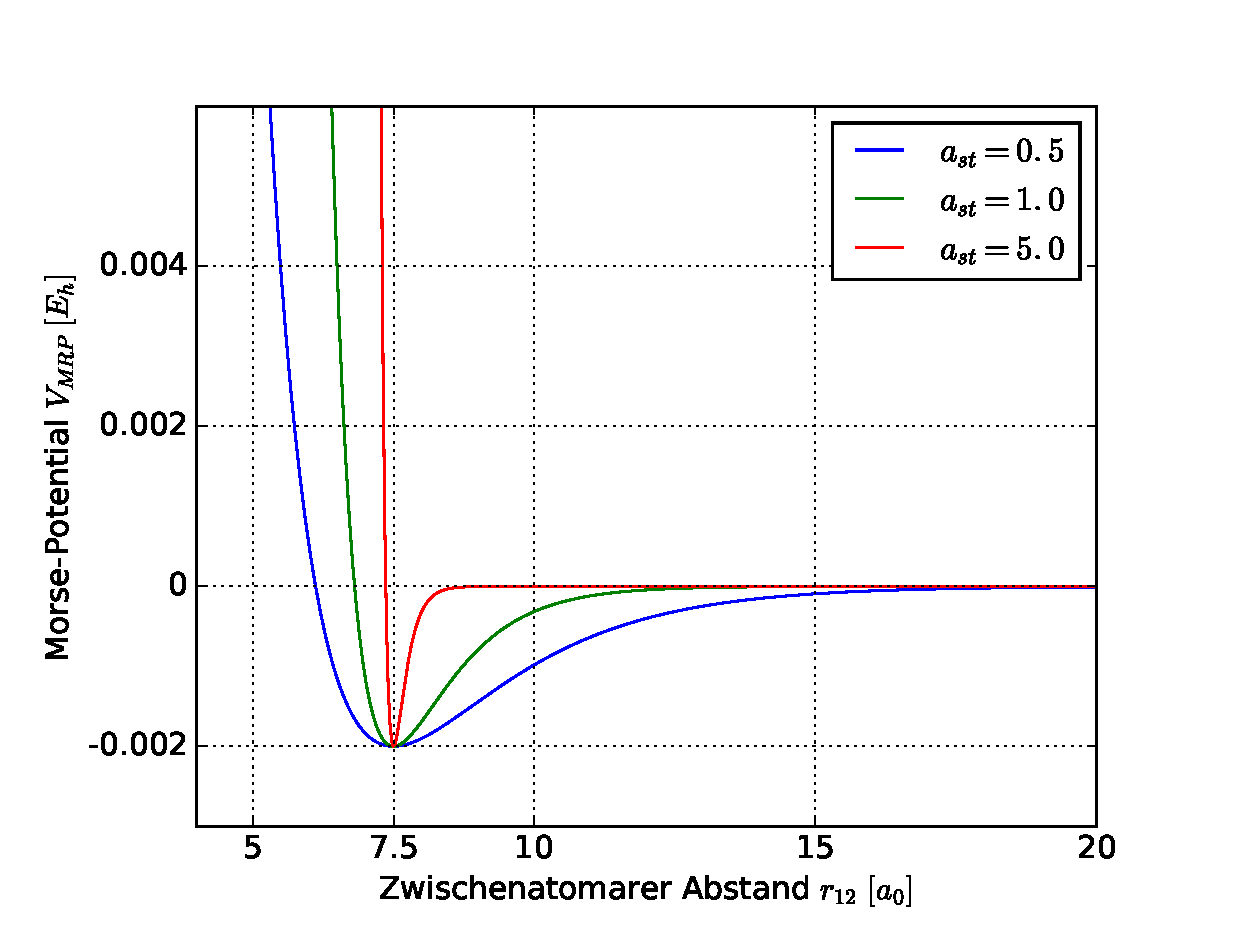
\includegraphics[scale=0.65]{MRP.eps}
%%	\vspace*{-10mm}
%	\caption{Es ist das Morse-Potential \ref{eq:MRP} mit fixierten Parametern 
%	$D_e = 0.002\ E_h$ und $R_m = 7.5\ a_0$ zu verschiedenen Exponenten 
%	$a_\text{st}$ im 
%	Bereich von 0.5 bis 5.0 dargestellt.}%TODO anderes Bild / vorallem andere 
%	%achsenbeschreiftungen !!!
%	\vspace{2mm} %\hrule 
%	\label{pic:MRP_1} 
%\end{figure}
%
Nun soll das Morsepotential als Funktion $f_{12}$ in das $\Pi^\pm_j$ - 
Integral  \ref{eq:PI-Integrale} eingesetzt werden:
%
\begin{align}
\Pi_j^\pm & =\int_{0}^{\infty}dr_{12}\ r_{12}^j \cdot V_\text{MRP}(r_{12}) \cdot
           e^{-\xi (r_{12} \pm Q)^2}\\
          & = \int_{0}^{\infty}dr_{12}\ r_{12}^j \cdot \rl{A_{\text{MRP}}\cdot 
          e^{-a_\text{st} r_{12}} + B_{\text{MRP}}\cdot e^{-2a_\text{st} 
          r_{12}}} \cdot e^{-\xi 
          (r_{12} \pm Q)^2} \\ \label{eq:PI_MRP}
          & = A^\prime_{\text{MRP}}\cdot \int_{0}^{\infty}dr_{12}\ r_{12}^j 
          \cdot e^{b_1\cdot r_{12} - \xi r_{12}^2} + B^\prime_\text{MRP}\cdot 
          \int_{0}^{\infty}dr_{12}\ r_{12}^j \cdot e^{b_2\cdot r_{12} - \xi 
          r_{12}^2}
\end{align}
%
Hierbei sind die Parameter $A^\prime_\text{MRP},\ B^\prime_\text{MRP},\ b_1$ 
und $b_2$ Zusammenfassungen von Konstanten. Diese sind durch
%
\begin{align}
A^\prime_\text{MRP}&:=A_\text{MRP}\cdot e^{-\xi Q^2}= D_e\cdot 
e^{2a_\text{st}R_m} \cdot 
e^{-\xi Q^2}\\
B^\prime_\text{MRP}&:=B_\text{MRP}\cdot e^{-\xi Q^2}= -2\cdot D_e\cdot 
e^{a_\text{st}R_m} 
\cdot e^{-\xi Q^2}\\
b_1 &:=-(a_\text{st}\pm 2\xi Q)\\
b_2 &:=-2(a_\text{st} \pm \xi Q )
\end{align}
%
definiert. Wie man an \ref{eq:PI_MRP} erkennt, kann das $\Pi^\pm_j$-Integral 
durch ein verallgemeinertes Integral über ein Monom des Grades j und einer 
Exponentialfunktion berechnet werden. Die Evaluation des Integraltyps
%
\begin{align}\label{eq:def:S}
S(\alpha,\beta,\gamma):=\int_{0}^{\infty}\ dx\ x^\alpha\cdot e^{\beta x - 
\gamma 
x^2}
\end{align}
%
wird im Abschnitt III.B-C der Arbeit \cite{av:1a} diskutiert. Für 
$\alpha\geq-1$, $\alpha\in \mathbb{N}, (\beta,\gamma)\in\mathbb{R}$ und $\gamma 
>0$  kann das Integral 
regulär berechnet werden. Für das MRP sind diese Forderungen immer 
erfüllt\footnote{da $\alpha=j$ wobei $j\in \mathbb{N}$ und $j\geq1$ mit 
$\beta=\{b_1,b_2\}$ und $\gamma=\xi$}, sodass das Integral ohne 
weitere Näherungen berechnet werden kann. $\Pi_j^\pm$ lässt sich damit 
also 
durch
%
\begin{align}\label{eq:PIinS_MRP}
\Pi^\pm_j=A^\prime_\text{MRP}\cdot 
S(j,b_1,\xi)+B^\prime_\text{MRP}\cdot 
S(j,b_2,\xi)
\end{align}
%
ausdrücken. In dieser Arbeit wird S mithilfe von 
%
\begin{align}\nonumber
S(\alpha,\beta,\gamma)  
&=(2\sqrt{\gamma})^{-\alpha-1}\Gamma(\alpha+1)\sqrt{\pi}\cdot
\left[\frac{M\rl{\frac{\alpha+1}{2},\frac{1}{2},\frac{\beta^2}{4\gamma}}}{\Gamma(\alpha/2+1)}
+\frac{\beta}{\sqrt{\gamma}} 
\frac{M\rl{\frac{\alpha}{2}+1,\frac{3}{2},\frac{\beta^2}{4\gamma}}}{\Gamma((\alpha+1)/2)}\right]\\\nonumber
%
&=\frac{1}{2}\, \gamma^{-1 - \frac{\alpha}{2}}\cdot \bigg[\beta\cdot 
\Gamma\rl{1 + \frac{\alpha}{2}}M\rl{1 + \frac{\alpha}{2}, \frac{3}{2}, 
\frac{\beta^2}{4\gamma}} \\ \label{eq:S,alpha>0}
&\qquad \qquad \qquad +\sqrt{\gamma}\cdot \Gamma\rl{\frac{1+\alpha}{2}}\cdot 
M\rl{\frac{1 + 
\alpha}{2}, 
\frac{1}{2},\frac{\beta^2}{4\gamma}} \bigg]
\end{align}
%
berechnet, wobei M Krummers konfluierte hypergeometrische Funktion ( auch mit 
$_1F_1$ bezeichnet) darstellt. Diese wird wiederum durch die 
Reihendarstellung 
%
\begin{align}\label{eq:reihe_M_kon.hyp.geo}
M(a,b,z)=1+\frac{az}{b}+\frac{(a)_2z^2}{(b)_2 
2!}+\dots +\frac{(a)_nz^n}{(b)_nn!}+\dots
\end{align}
mit den Pochhammer-Symbol
\begin{align}
(a)_n=a(a+1)(a+2)\dots(a+n-1), \ (a)_0=1
\end{align}
% 
berechnet (vergleiche mit \cite{b:1a} und \cite{b:6a}).\\
Erwähnt werden muss an dieser Stelle, dass \cite{av:1a} eine leicht andere 
Formel verwendet wird. In dieser Stelle findet Tricomis 
konfluierte 
hypergeometische Funktion 
($\mathcal{U}$) ihre Anwendung. Jedoch kann mit den im 
Vorfeld benutzten 
Konversionen  ( Definition (57) = Formel \ref{eq:def:S} ) die entsprechende 
Gleichung (60) aus \cite{av:1a} nicht abgeleitet werden\footnote{Es 
konnte 
sogar mithilfe eines kleinen MATHEMATICA-Skrips gezeigt werden, dass 
die linke 
Seite nicht der rechten entspricht. Durch Änderung der Definition 
\ref{eq:def:S} ($\beta\rightarrow-\beta$) und Vergleich mit 
\cite{b:6a} kann 
eine beinahe Übereinstimmung gefunden werden, jedoch müsste 
diese noch 
genauer 
geprüft und alle darauf folgenden Gleichungen in \cite{av:1a} 
angepasst werden. 
In dieser Arbeit wird diese Korrektur nicht weiter 
verfolgt.}. 
Dementsprechend wird 
auch nicht, der im unterstützenden Material \cite{av:1a2} 
dargestellte 
Weg zur Berechnung von $\mathcal{U}$ verwendet. Dieser berechnet $\mathcal{U}$ 
in verschiedenen Intervallen mit jeweils anderen Formeln, um die Konvergenz und 
Genauigkeit zu verbessern. Daher ist zu erwarten, dass auch 
\ref{eq:S,alpha>0} nicht für alle Bereiche der Parameter numerisch stabile 
Ergebnisse liefert\footnote{Es wird auch eine Integration 
durch quadratische 
Ergänzung des Exponenten und anschließender Umformung auf eine Erf-Funktion 
bzw. unvollständige $\Gamma$-Funktion 
versucht. Jedoch liefert dieses Vorgehen eine zu ungenaue 
Berechnung, da bei 
der auftretenden Subtraktion $1-\text{Erf}(x)$ schnell 
signifikante Stellen verloren gehen.}. Getestet wird diese Erwartung in Kapitel 
\ref{sec:Implementierung}. % (??) 
%
%
%
\subparagraph{Das Lennard-Jones-Potential} hat vor allem zwei gängige 
Darstellungen. Es muss erwähnt werden, dass in dieser Arbeit das sogenannte 
(12,6)-LJP benutzt wird:
%
\begin{align}\label{eq:def:LJP}
V_{\text{LJP}}(r_{12})&=D_e\cdot\left[ \rl{\frac{R_m}{r_{12}}}^{12} - 
2\rl{\frac{R_m}{r_{12}}}^6 \right]\\
                      &= 
                      \frac{A_\text{LJP}}{r_{12}^{12}}+\frac{B_\text{LJP}}{r^6_{12}}
                       \quad.
\end{align}
$D_e$ und $R_m$ sind analog zum MRP definiert. Auch $A_\text{LJP}$ und 
$B_\text{LJP}$ sind Zusammenfassungen von Konstanten:
%
\begin{align}
A_\text{LJP} &= D_e\cdot R_m^{12} \\
B_\text{LJP} &= -2\cdot D_e \cdot R_m^6 
\end{align}
%
Die Potenzen 12 bzw. 6 entstehen durch die betrachtete Wechselwirkung und 
Eigenschaften der Teilchen. Für neutrale, homonukleare Atome entsteht die 
Van-der-Waals Anziehung, die gut durch eine inverse sechste 
Potenz beschrieben 
werden kann. Der hier verwendete abstoßende Term mit der 
zwölften Potenz ist die
Konversion und kann im Zweifelsfall noch variiert werden. Im Gegensatz zum MRP 
hat das LJP in dieser Form keinen weiteren freien Parameter.\\
Für das $\Pi^\pm_j$-Integral ergibt sich:
%
\begin{align}
\Pi_j^\pm & =\int_{0}^{\infty}dr_{12}\ r_{12}^j \cdot V_\text{LJP}(r_{12}) \cdot
             e^{-\xi (r_{12} \pm Q)^2}\\\nonumber
          & = \int_{0}^{\infty}dr_{12}\ r_{12}^j \cdot 
          \rl{\frac{A_\text{LJP}}{r_{12}^{12}}+\frac{B_\text{LJP}}{r^6}}\cdot
          e^{-\xi (r_{12} \pm Q)^2}\\\nonumber
%\end{align}
%\begin{align}
%\Pi_j^\pm 
& = A^\prime_\text{LJP}\int_{0}^{\infty}dr_{12}\ r_{12}^j \cdot 
\frac{1}{r_{12}^{12}}\cdot e^{\mp 2\xi Q r_{12} -\xi r_{12}^2}+ 
B^\prime_\text{LJP}\int_{0}^{\infty}dr_{12}\ r_{12}^j 
\cdot\frac{1}{r_{12}^6}\cdot e^{\mp 2\xi Q r_{12} -\xi 
r_{12}^2}\\\nonumber
&=A^\prime_\text{LJP}\int_{0}^{\infty}dr_{12}\ r_{12}^{j-12}\cdot e^{\mp 2\xi Q 
r_{12} -\xi r_{12}^2}+ 
B^\prime_\text{LJP}\int_{0}^{\infty}dr_{12}\ r_{12}^{j-6}\cdot e^{\mp 2\xi Q 
r_{12} -\xi r_{12}^2}\\\label{eq:PI_LJP}
&=A^\prime_\text{LJP}\cdot 
S(\alpha_1,\beta,\gamma)+B^\prime_\text{LJP}\cdot 
S(\alpha_2,\beta,\gamma)\ .
\end{align}
%
Es ist zu erkennen, dass auch mit dem LJP  sich das $\Pi^\pm_j$-Integral auf 
den Typ \ref{eq:def:S} vereinfachen lässt. In diesem Fall gelten die 
Definitionen 
%
\begin{align}\nonumber
A^\prime_\text{LJP}:=A_\text{LJP}\cdot e^{-\xi Q^2} &\quad,\quad 
B^\prime_\text{LJP}:=B_\text{LJP}\cdot e^{-\xi Q^2} \\\nonumber
\alpha_1:=j-12 &\quad,\quad \alpha_2:=j-6 \\\nonumber
\beta&=\mp 2\xi Q\\
\gamma &= \xi \qquad,
\end{align}
wobei jedoch nun $\alpha$ auch eine negative ganze Zahl sein kann, da 
$j\geq1$ ist.  Die Integrale mit positiven $\alpha$ können analog zu 
\ref{eq:S,alpha>0} berechnet werden. Dagegen können die Integrale mit 
negativem $\alpha$ nicht regulär bestimmt werden. Sie sind divergent, da der 
Integrand einen Pol in 0 besitzt. Wie oben schon einmal erwähnt, ist eine 
Divergenz in 0 nicht überraschend, da die Gauß-Funktionen die Randbedingung in 
0 nicht erfüllen. Physikalisch gesehen ist jedoch eine Divergenz nicht 
realistisch (es könnte auch eine divergente Energie folgen). 
Dementsprechend kann eine Renormierung versucht werden. \cite{av:1a} schlägt in 
Abschnitt III.A. bzw. III.C. ein Renormierungsschema vor.\\
Hier zeigt sich eine entscheidende Schwäche des LJP als Näherungsfunktion. 
%
%
%
\subparagraph{Das Renormierungsschema} \label{sec:renorm}
%
soll auf Integrale des Typs 
%
\begin{align}\label{eq:def:T-Int}
T_s^\pm(x)&:=\mathcal{R}\int_{0}^{\infty}\frac{dz}{z^s}e^{\pm z-xz^2}
\end{align}
%
angewendet werden, welche dem besprochenen Fall von negativen 
$\alpha$ 
entsprechen. $\mathcal{R}$ steht dabei für die Anwendung einer 
Renormierung. 
Mit den Definitionen 
%
\begin{align}
s=-\alpha \qquad\text{und} \qquad x=\frac{\gamma}{\beta^2} 
\end{align} 
%
folgt der Zusammenhang 
%
\begin{align}\label{eq:SinT}
S(\alpha,\beta,\gamma)&=|\beta|^{-\alpha-1}T_{-\alpha}^{\text{sign} 
(\beta)}(\gamma/\beta^2) \qquad.
\end{align}
%
Das Schema entspricht folgendem Vorgehen: Die Integrale 
werden zunächst analytisch 
von $\epsilon$, anstatt von 0, bis $\infty$ berechnet, anschließend in eine 
Reihe in $\epsilon$ entwickelt und alle divergenten\footnote{bzgl. 
$\epsilon\rightarrow0$} Terme entfernt. Für $\epsilon\rightarrow0$ bleibt dann 
nur noch der Term übrig, der keine $\epsilon$ Abhängigkeit hat. Dieser wird 
dann als Ergebnis des Integrals gewertet. Nach Angaben der Autoren von 
\cite{av:1a} scheint dieses Schema plausible Werte zu liefern.\\
Um nun $T_s$ möglichst effizient zu berechnen, zeigt \cite{av:1a}, dass die 
Rekursion
%
\begin{align}\label{eq:recursivT}
s\cdot T^\pm_{s+1}(x)&=\pm\sum_{l=0}^{s/2}\frac{(-x)^l}{l!(s-2l)!}\pm 
T^\pm_{s}(x)-2xT^\pm_{s-1}(x)
\end{align}
%
gilt\footnote{Gleichung (68) aus \cite{av:1a}, das Analogon zu 
\ref{eq:recursivT} bzgl. S, hat einen Tippfehler: Vor dem 
Summenzeichen soll 
ein zusätzlicher Faktor $-\frac{1}{\alpha}$ stehen. }. Ausgehend davon müssen 
zuerst zwei Integrale gelöst werden, um die Rekursion zu starten. $T_0^\pm$ 
kann durch elementarer Integration über eine Gaußfunktion  zu 
%
\begin{align}\label{eq:T0}
T_0^\pm(x) = \sqrt{\frac{\pi}{4x}}e^{\frac{1}{4x}}\left[1\pm 
\text{Erf}\rl{\frac{1}{2\sqrt{x}}}\right]
\end{align}
%
bestimmt werden\footnote{Gleichung (70) in \cite{av:1a} hat einen Tippfehler; 
Gleichung \ref{eq:T0} zeigt die korrigierte Version. }. Das zweite benötigte 
Integral $T^\pm_1$ ist aufwendiger zu berechnen. Dabei hat das Ergebnis von 
\cite{av:1a} (Gleichung (72)) einen etwas größeren Tippfehler. Dementsprechend 
wird nun eine verkürzte Ableitung gezeigt, um überzeugend die 
Richtigkeit des 
hier präsentierten Integrals darzustellen. Dafür wird die Definition ( 
Gleichung (71) aus \cite{av:1a} )
%
\begin{align}\label{eq:def:omega}
\omega_k(x):=\int_{0}^{\infty}dz\ z^k\log(z)e^{-xz-z^2}
\end{align}
%
benötigt. Betrachtet man nun $T_1^\pm$ und führt eine partielle Integration 
durch, folgt:
%
\begin{align*}
T_1^\pm (x)=& \mathcal{R}\int_{0}^{\infty} \frac{dz}{z} \ e^{\pm z - xz^2}\\
           =&\epsilon\overset{\mathcal{R}}{\rightarrow}0
           \int_{\epsilon}^{\infty} \frac{dz}{z} \ e^{\pm z - xz^2}\\
\overset{\text{part. Int.}}{=}&\epsilon\overset{\mathcal{R}}{\rightarrow}0 
\rl{\log(z)e^{\pm z-xz^2}|_{z=\epsilon}^\infty - 
\int_{\epsilon}^{\infty}\log(z)e^{\pm z-xz^2} \cdot (\pm 1-2xz)}\quad,
\end{align*}
%
wobei "$\epsilon\overset{\mathcal{R}}{\rightarrow}0$"\ das oben 
beschriebene Renomierungsschema andeuten soll. Die ersten beiden Terme 
entfallen; einer wird 0 durch Einsetzten der Grenze, der andere ist ein zu 
renormierender Term und entfällt somit. Dadurch verschwindet hier die 
Divergenz. An dem verbleibenden Integral 
wird die Substitution $z=\frac{u}{\sqrt{x}}$ durchgeführt. Nach der Trennung 
des Logarithmus mit $\log\rl{\frac{u}{\sqrt{x}}}=\log(u)-\log(\sqrt{x})$ und 
Integration über alle entstehenden Gauß-Funktionen und 
anschließenden Vergleich 
mit der Definition \ref{eq:def:omega} folgt:
%
\begin{align}\label{eq:korr_T_1}
T_1^\pm(x)= \mp \frac{1}{\sqrt{x}} \omega_0(\pm \frac{1}{\sqrt{x}}) + 2\ 
\omega_1(\pm\frac{1}{\sqrt{x}})-\frac{1}{2}\log(x) \qquad.
\end{align}
%
Im Anhang \ref{sec:AnhangB:T_Integral} ist eine detailliertere Herleitung 
angeheftet. Die verbleibenden Berechnungen der Funktionen $\omega(x)_k$ können 
über
%
%\begin{align*}
%\omega_k(x)=\begin{cases}
%\sum_{k=0}^{\infty}\frac{(-x)^k}{k!}\frac{1}{4}\Gamma\rl{\frac{k+1}{2}}\psi_d\rl{\frac{k+1}{2}}&,
%k=0\\
%\sum_{k=0}^{\infty}\frac{(-x)^k}{k!}\frac{1}{4}\Gamma\rl{\frac{k}{2}+1}\psi_d\rl{\frac{k}{2}+1}&,
%k=1\\
%\end{cases}
%\end{align*}
%
Reihenentwicklungen für verschiedene Größenordnungen von x  
%   
durchgeführt werden (vergleiche dazu \cite{av:1a2} und Anhang
\ref{sec:AnhangB:T_Integral}). 
%Hierbei ist $\psi_d$ die Diagammafunktion, welche für 
%ganze 
%und halbe Zahlen durch
%
%\begin{align*}%\label{eq:def:diagamma}
%\psi_d\rl{n+\frac{1}{2}}&=-\gamma_E-2\log2+\sum_{k=1}^{n}\frac{2}{2k-1}\\
%\psi_d(n)&=-\gamma_E+\sum_{k=1}^{n-1}\frac{1}{k}
%\end{align*}
%
%mit $n\in \mathbb{N}$ berechnet werden kann. $\gamma_E$ ist die 
%Euler-Mascheroni-Konstante. 

Damit sind alle Informationen zur 
Berechnung von $T_1^\pm$ bekannt. \cite{av:1a} gibt noch zu bedenken, dass 
\ref{eq:recursivT} nur für $x>1$ mit hoher Genauigkeit verwendet werden kann 
und für x<1 numerisch instabil wird. Daher schlägt \cite{av:1a} vor, bei einem 
sehr hohen Wert\footnote{"\ Signifikant"\ größer als das zu berechnende s, 
Tests 
zeigen für s=7 sollte man min. bei $s_{max}=28$ angefangen.} $s_{max}$ 
die Integrale $T_{s_{max}+1}^\pm=0$ und $T_{s_{max}}=1$ zu 
setzen und die 
Rekursion \ref{eq:recursivT} für absteigende s auszuwerten, 
das heißt
%
\begin{align}\label{recursiveT2}
T^\pm_{s-1}(x)=\frac{1}{2x}\cdot 
\left[\pm\sum_{l=0}^{s/2}\frac{(-x)^l}{l!(s-2l)!}\pm T^\pm_s(x)-s\cdot 
T^\pm_{s+1}\right]
\end{align}
%
zu benutzen. Jedoch müssen die Integrale nachskaliert werden. 
Dazu wird die 
Rekursion bis s=0 durchgeführt und das Ergebnis mit dem analytischen Wert für 
$T_0^\pm$ \ref{eq:T0} verglichen. Anschließend werden alle Integrale mit dem 
Quotienten
%
\begin{align*}
k=\frac{\rl{T_0^{\pm}}^*}{\rl{T_0^\pm}^{**}}
\end{align*}
%
multipliziert. Dabei ist  * der analytische Wert aus \ref{eq:T0} und ** das 
Ergebnis 
der letzten Rekursion.\\
Dieses Vorgehen birgt auch eine gewisse numerische Instabilität, die auch in 
Kapitel \ref{sec:Implementierung} genauer betrachtet 
wird.%??check?? %checken, 
%dass auch wirklich dieser Abschnitt diskutiert wurde. 
%
%
%
\subsubsection{Zusammenfassung und Vergleich}
%
Durch Verwendung einer Näherungsfunktion für das Wechselwirkungspotential 
zwischen zwei neutralen Atomen kann das Basisintegral, des im Abschnitt 
\ref{sec:Algorithmus} beschriebenen Algorithmus, mittels 
analytischer 
Formeln, Rekursionsrelationen und wohl bekannter numerischer Funktionen, wie 
zum Beispiel der Erf-Funktion oder der $\Gamma$-Funktion, berechnet werden. 
Vorgestellt ist das MRP und das LJP. Die folgende Darstellung zeigt beide 
Potentiale im Vergleich zueinander und zu einem numerischen Potential aus 
\cite{phdthesis:sergey}.
%
%\begin{figure}[H] \centering
%	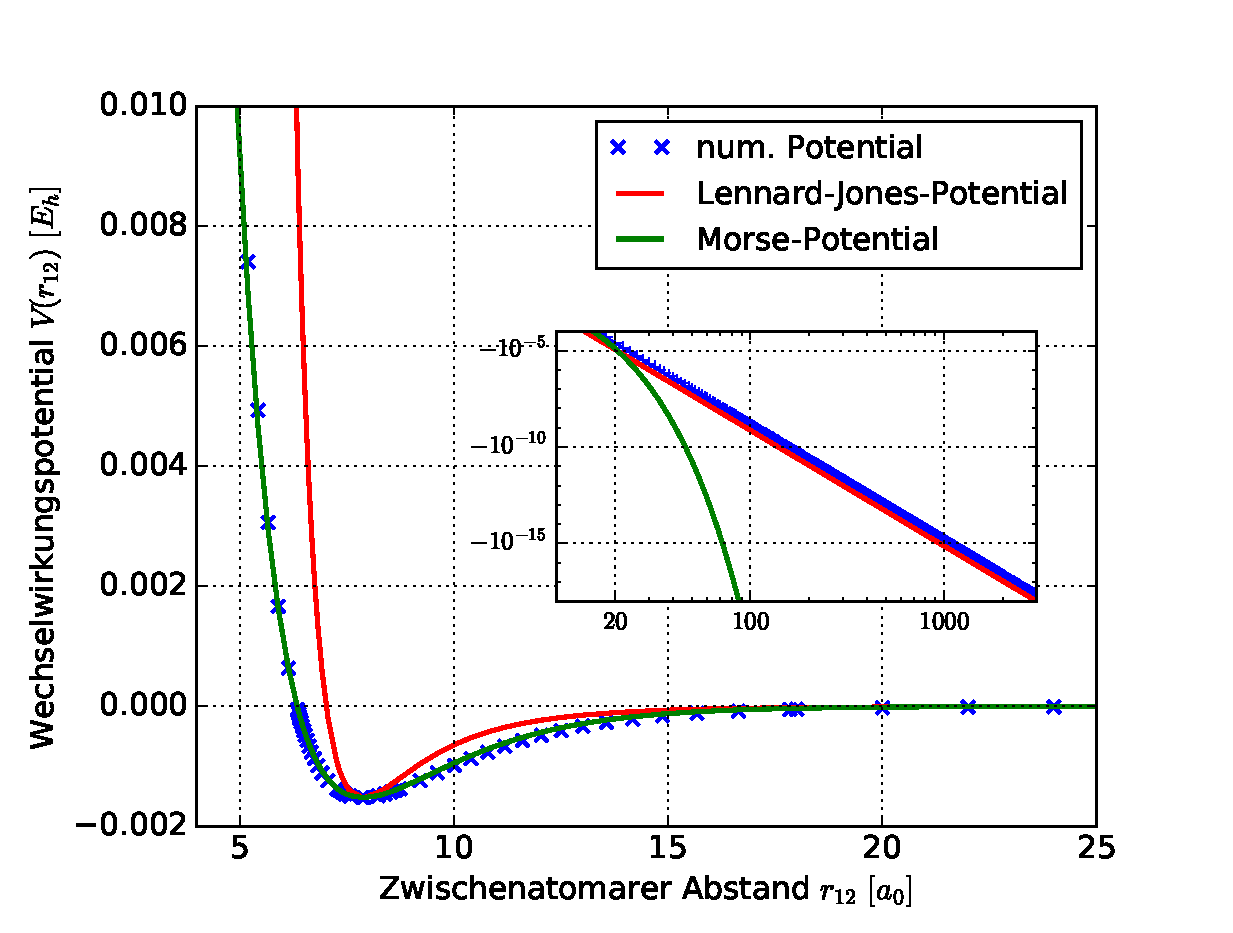
\includegraphics[scale=0.7]{WW.eps}
%	%	\vspace*{-10mm}
%	\caption{Dargestellt ist ein numerisches Potential (blau, gekreuzt) eines 
%	angeregten Tripletzustandes des $^7$Li$^7$Li Systems und 
%	zwei 
%	Näherungsfunktionen: das Morse-Potential (grün) und das 
%	Lennard-Jones-Potential (rot). Im Sub-Plot sieht man das Verhalten für 
%	größere Abstände. Für die Parameter $D_e$ (Dissoziationsenergie) und $R_m$ 
%	(Lage des Minimuns) ist der Tiefpunkt der 
%	numerischen Kurve benutzt worden. Der Exponent des MRPs 
%	wird zu 
%	$a_\text{st}=0.45$ 
%	gewählt.}
%	%\vspace{2mm} %\hrule 
%	\label{pic:Pot} 
%\end{figure}
%
In \ref{pic:Pot} ist zu sehen, dass das MRP im Bereich von 5-20 $a_0$ eine sehr 
gute Näherung 
darstellt, wogegen das LJP in diesem Bereich kaum dem numerischen Potential 
folgt. Für Abstände größer als 20 $a_0$ hingegen fällt das 
MRP deutlich zu 
schnell ab. Schon bei einem Abstand von ungefähr 100 $a_0$ erreicht es schon 
die Rechnergenauigkeit und wird auf 0 gerundet. Das LJP nähert sich dagegen der 
numerischen Kurve weiter an und 
folgt der Kurve 
über mehrere Größenordnungen des Abstandes. Lediglich ein leichter Off-set ist 
zu erahnen. An dieser Stelle sei erwähnt, dass die hier 
dargestellte Näherung 
nur durch optische Anpassung gewonnen wird. Es ist zu 
erwarten, dass eine 
numerische Anpassung (Fit) ein besseres Ergebnis auf Kosten 
einer 
Nichtübereinstimmung im Minima liefern kann.  \\

Das MRP besitzt den großen Vorteil einer vollständigen Beschreibung und 
Berechnung ohne den Bedarf einer Renormierung. Dagegen beschreibt das LJP die 
physikalische Gegebenheit besser und für große Abstände auch quantitativ 
genauer. Mithilfe des freien Parameters im Exponenten 
kann jedoch das MRP die Kurve nahe am Ursprung besser beschreiben. \\

Ziel der Betrachtung ist es, die Bemühung einer Renomierung des bekannten 
$\delta$-Pseudopotentials als Wechselwirkungspotential zu umgehen, indem ein 
realistisches Potential verwendet wird. Erhofft wird eine bessere Berechnung 
mittels CI von ultrakalten Gasen. Durch Nutzung des LJP und 
des 
Algorithmus kann zwar ein realistisches bzw. 
realistischeres\footnote{da das 
LJP dennoch eine Näherungsfunktion ist} Potential als das 
$\delta$-Potential 
verwendet werden, jedoch auf Kosten einer neuen 
Renormierung\footnote{Renormierung der Basisintegrale}. Dementsprechend 
erfüllt das LJP nicht ganz die erwarteten Eigenschaften. 
Dagegen ist das MRP 
mathematisch angenehmer und es ist keine Renormierung nötig. \\
Das MRP ist ebenfalls ein realistischeres Wechselwirkungspotential als das 
$\delta$-Potential, auch wenn es für große Abstände deutlich zu schnell 
abfällt. 
Dennoch soll es möglich sein, die relevanten Eigenschaften 
mittels MRP 
darzustellen und herauszufinden, ob eine CI-Rechnung 
prinzipiell möglich sei 
und ob diese eine Verbesserung liefere. Das MRP divergiert 
zwar nicht in 0, 
nimmt aber sehr große Werte an. Es kann daher passieren, dass im Rahmen der 
Integration zwar Ergebnisse produziert werden, diese aber unphysikalisch groß 
sind. Dieses Verhalten muss durch geeignete Wahl der Basisfunktionen der 
CI-Rechnung berücksichtigt werden.   \\

Weiterhin sei hier erwähnt, dass es auch Mischformen dieser Potentiale gibt. 
Vorstellbar ist, dass das Potential
%
\begin{align}
V\propto e^{-a_\text{st}\cdot r}-\rl{\frac{R_m}{r}}^6 \quad,
\end{align}
%
auch (modifiziertes) Buckingham-Potential genannt (siehe z.B. in \cite{av:2b} 
oder 
\cite{av:3b}), eine noch bessere 
Beschreibung über den gesamten Bereich der Abstände liefert und die guten 
Eigenschaften beider Potentiale vereint. Ohne weitere Untersuchung kann auf 
zwei Tatsachen hingewiesen werden: Zum einen muss auch dieses 
Potential für 
einige Fälle im Rahmen des oben beschriebenen Algorithmus renormiert werden, 
jedoch seltener als das LJP. Zum anderen 
beinhaltet dieses Potential den $\frac{1}{r^6}$ -Term und wird daher die 
Eigenschaft des LJP erben, sodass große Abstände gut 
beschrieben werden können.
%
%
%